\documentclass{article}
\usepackage{graphicx} % Required for inserting images
\usepackage[
backend=biber,
style=numeric,
sorting=ynt
]{biblatex}
\usepackage{todonotes}
\usepackage{caption}
% \usepackage{fontspec}

% \setmainfont{Times New Roman}

\addbibresource{bibliography.bib}

\title{Making A Roguelike Engine with SvelteKit}
\author{Kutay Güler}
\date{December 2023}

\begin{document}

\maketitle
\tableofcontents

\section{Introduction}
In every software project, whether it is a game, a game engine or a simple web application, there is a property which can cause a project to get derailed or follow a steady pace to its ultimate destination, and that property is called “scale.” 

Although getting derailed is a negative phrase, in the context of software engineering it could be a necessity, especially for game engines. Most popular game engines today have massive codebases with many people working on them, because their promise is the ability to create any type of game at any scale with only one tool. This is like inventing a train that can fly, travel underwater, go to the moon and of course, slide on iron rails. By its nature, it should derail from time to time. 

It sounds like there are only upsides to this invention since it can go anywhere but upon closer inspection, we can conclude that it is incorrect. The different environments this train will travel through will require many edge cases which will increase the literal size of the train and its maintenance cost. As for passengers, the experience will require some time to get used to and first timers will be definitely intimidated. 

This project’s aim is to create a straightforward train with its blueprints open to the public, that is, an open-source game engine specifically designed for roguelikes. The target audience is people who want to make roguelike games without having to learn coding but there will be grounds for programmers too. 

\subsection{Roguelike}
The term roguelike originated in a forum discussion to find an umbrella term for games that were similar to each other at the time. After three weeks of discussion, the “granddaddy of these games” Rogue, was appended with “-like” suffix to turn it into a game genre that we still use today \cite{roguelike-term}. 

Many roguelike games were released in the upcoming years, so it was time to define what a roguelike game is more concretely. In 2008, the International Roguelike Development Conference was held in Berlin, and gave birth to the Berlin Interpretation \cite{berlin}.

\subsection{Berlin Interpretation}

Text below is the formatted version of the original Berlin Interpretation text. All the content has been kept exactly the same.

\subsection*{Preamble}

This definition of "Roguelike" was created at the International 
Roguelike Development Conference 2008 and is the product of a 
discussion between all who attended. The definition at 
http://www.roguetemple.com/roguelike-definition/ was used as the 
starting point for the discussions. Most factors are newly phrased, 
new factors have been added, some factors have been removed.

\subsection*{General Principles}
 
"Roguelike" refers to a genre, not merely "like-Rogue". The genre is 
represented by its canon. The canon for Roguelikes is ADOM, Angband, 
Crawl, Nethack, and Rogue. 
 
This list can be used to determine how roguelike a game is. Missing 
some points does not mean the game is not a roguelike. Likewise, 
possessing some points does not mean the game is a roguelike.  
 
The purpose of the definition is for the roguelike community to better 
understand what the community is studying. It is not to place 
constraints on developers or games. 

\subsection*{High value factors}
\begin{itemize}

\item\textbf{Random environment generation:}
The game world is randomly generated in a way that increases 
replayability. Appearance and placement of items is random. 
Appearance of monsters is fixed, their placement is random. 
Fixed content (plots or puzzles or vaults) removes randomness. 

\item\textbf{Permadeath:} 
 You are not expected to win the game with your first character. You 
start over from the first level when you die. (It is possible to save 
games but the savefile is deleted upon loading.) The random 
environment makes this enjoyable rather than punishing. 

\item\textbf{Turn-based:}
Each command corresponds to a single action/movement. The game is not 
sensitive to time, you can take your time to choose your action.   

\item\textbf{Grid-based:} 
The world is represented by a uniform grid of tiles. Monsters (and 
the player) take up one tile, regardless of size. 

\item\textbf{Non-modal:} 
Movement, battle and other actions take place in the same mode. Every 
action should be available at any point of the game. Violations to 
this are ADOM's overworld or Angband's and Crawl's shops. 

\item\textbf{Complexity:} 
The game has enough complexity to allow several solutions to common 
goals. This is obtained by providing enough item/monster and item/item 
interactions and is strongly connected to having just one mode. 

\item\textbf{Resource management:} 
You have to manage your limited resources (e.g. food, healing potions) 
and find uses for the resources you receive. 

\item\textbf{Hack'n'slash:}
Even though there can be much more to the game, killing lots of 
monsters is a very important part of a roguelike. The game is player- 
vs-world: there are no monster/monster relations (like enmities, or 
diplomacy).  

\item\textbf{Exploration and discovery:} 
The game requires careful exploration of the dungeon levels and 
discovery of the usage of unidentified items. This has to be done anew 
every time the player starts a new game.

\end{itemize}

\subsection*{Low value factors} 
\begin{itemize}
    \item \textbf{Single player character:}
    The player controls a single character. The game is player-centric, 
    the world is viewed through that one character and that character's 
    death is the end of the game. 
    
    \item \textbf{Monsters are similar to players:}
    Rules that apply to the player apply to monsters as well. They have 
    inventories, equipment, use items, cast spells etc. 
    
    \item \textbf{Tactical challenge:}
    You have to learn about the tactics before you can make any 
    significant progress. This process repeats itself, i.e. early game 
    knowledge is not enough to beat the late game. (Due to random 
    environments and permanent death, roguelikes are challenging to new 
    players.) 
    
    The game's focus is on providing tactical challenges (as opposed to 
    strategically working on the big picture, or solving puzzles). 
    
    \item \textbf{ASCII display:}
    The traditional display for roguelikes is to represent the tiled world 
    by ASCII characters. 
    
    \item \textbf{Dungeons:}
    Roguelikes contain dungeons, such as levels composed of rooms and 
    corridors. 
    
    \item \textbf{Numbers:}
    The numbers used to describe the character (hit points, attributes 
    etc.) are deliberately shown. 
\end{itemize}

\section{Existing Solutions}
\subsection{Godot, Unity and Unreal}
These are the top three game engines for any genre. They are not specifically designed for roguelikes and have a longer learning process for the user since all of them require coding visually or manually \cite{godot}\cite{unity}\cite{unreal}.

\subsection{RPGMaker}
RPGMaker as the title suggests, is not an engine for roguelikes but our design decisions are similar. RPGMaker is an engine for RPGs (role playing games), and it has a low code environment, and it is the main inspiration for Roguelighter \cite{rpgmaker}.  

However, unlike Roguelighter, RPGMaker is proprietary software, and it has a UI layer for game data. Roguelighter has no UI for game data which eliminates any UI related issues that can arise like accessibility, readability, or consistency. 
 
Unity and Unreal is even used outside of game development industry. Their products are used in automobiles, architecture, engineering, and the film industry \cite{unity}\cite{unity-industry}\cite{unreal}.

\section{Technology}
\subsection{Svelte and SvelteKit}
Svelte is a JavaScript framework that leans on simplicity and performance with the power of its compiler-based architecture. An average Svelte project will have less lines of code and bundle size compared to its counterparts like React, Angular and Vue. Which makes it easier to maintain \cite{svelte-less}.

% TODO: change this description
SvelteKit is a full-stack application framework for Svelte. Although this project is not necessarily a full-stack application, a built-in router might be useful in the future, in case the software requires multiple views \cite{sveltekit}.

\subsection{WebGL}
WebGL (Web Graphics Library) is a JavaScript API for rendering high-performance interactive 3D and 2D graphics within any compatible web browser without the use of plug-ins. WebGL does so by introducing an API that closely conforms to OpenGL ES 2.0 that can be used in HTML canvas elements. This conformance makes it possible for the API to take advantage of hardware graphics acceleration provided by the user's device \cite{webgl}. 

\subsection{ThreeJS}
ThreeJS is a canvas library which provides primitives and abstractions on top of WebGL to make building 3D projects faster, more readable, and more maintainable \cite{threejs}.

\subsection{Threlte}
Threlte is a declarative library built on top of ThreeJS. Instead of writing imperative code with ThreeJS, developers are allowed to write declarative component-based code to describe their 3D scenes \cite{threlte}.

\subsection{TypeScript}
\todo{write typescript description and features}

\subsection{HOTScript}
HOTScript is a library of composable functions for types. It uses generics to compose function-like behavior inside TypeScript’s type system \cite{hotscript}.

\subsection{TailwindCSS}
TailwindCSS is a utility-first CSS library that provides atomic classes which only affect a single CSS property . This atomic approach is inline with Roguelighter's philosophy: Locality of Behavior\cite{tailwindcss}.

\subsection{Monaco Editor}
Monaco Editor is an open source, fully featured, browser-based code editor. It is the editor that powers Visual Studio Code, which is the most popular integrated development environment as of today \cite{monaco-editor}\cite{developer-survey}.

\subsection{Tauri}
Tauri is a framework for building tiny and fast binaries for all major desktop platforms. Developers can integrate any front-end framework that compiles to HTML, JS and CSS for building their user interface. The backend of the application is a rust-sourced binary with an API that the front-end can interact with \cite{tauri}.

\subsection{TypeDoc}
TypeDoc is a documentation generator for TypeScript type declarations. It uses declarations themselves and TSDoc comments placed above the declarations to generate documentation in JSON or in multi page HTML format \cite{typedoc}.

\section{Architecture}
Roguelighter consists of a library and two apps. The library is the engine itself, and the apps are a desktop application and a website which includes documentation, interactive tutorial and download link for the desktop app. Library code is shared between these two projects with monorepo architecture.

\subsection{Monorepo}
Explaining monorepos can be easier if we first learn what is the opposite of a monorepo which we can name as polyrepos. A polyrepo is the current standard way of developing applications: a repo for each team, application, or project. And it's common that each repo has a single build artifact, and simple build pipeline. This approach brings autonomy to different teams working on the same project but it has its downsides.\\

First off, sharing code becomes cumbersome. The consumer repo should have a dependency to the provider repo and consumers should wait for the latest updates to go live to use a certain feature. Common code patterns and components gets implemented in each repo differently, which increases the maintenance cost for each team and creates duplicate logic. Tooling becomes inconsistent, as each team introduces their own standards or ad hoc solutions.\\

So what is a monorepo? A monorepo is a single repository containing multiple distinct projects, with well-defined relationships. No need to publish packages since all the consumers are in the same repo. No need to worry about incompatibilities because of projects depending on conflicting versions of third party libraries. Everything related to the monorepo becomes consistent whether that is a simple component, a developer tool or a complex build workflow \cite{monorepo}.

\subsection{Desktop Application}
\subsubsection{Configuration File}

\begin{itemize}
    \item \textbf{Settings:} Provides defaults for the project. Such as default frames per second, default animation function and default animation duration.
    \item \textbf{Backgrounds:} An object where keys define the name of the background, and value points to the route of the source. This object also affects the Map Editor interface, which we will see in \todo{reference}\\\\
    \begin{minipage}{\linewidth}
        \centering
        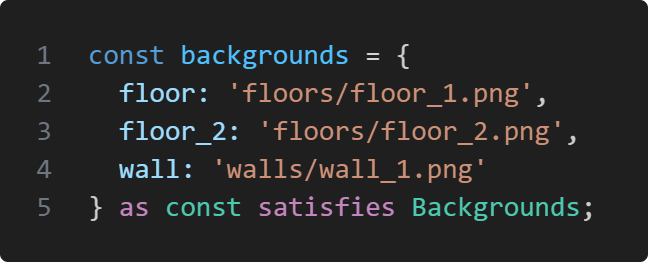
\includegraphics[width=1\textwidth]{backgrounds.png}
        \captionof{figure}{Example Backgrounds object}
        \label{fig:figure1}
    \end{minipage}

    \item \textbf{Collisions:} An array of background keys. This tells the game that agents cannot move into tiles with these backgrounds.\\\\
    \begin{minipage}{\linewidth}
        \centering
        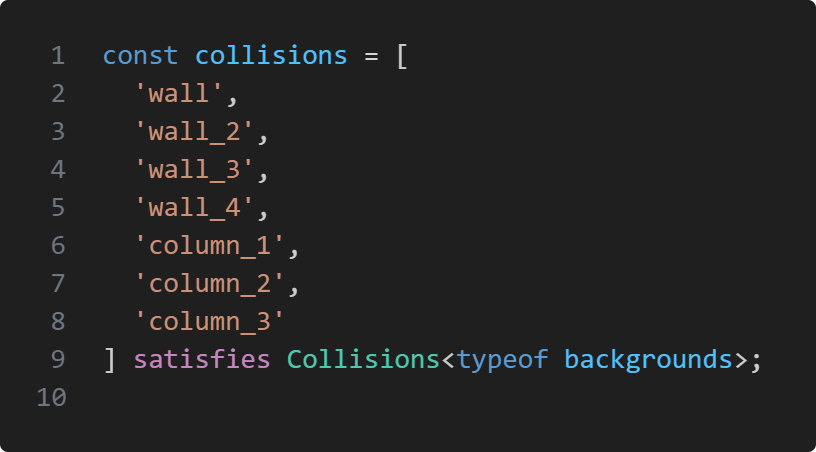
\includegraphics[width=1\textwidth]{collisions.png}
        \captionof{figure}{Example Collisions object}
        \label{fig:figure2}
    \end{minipage}
    
    \item \textbf{Agents:} Agents are player and non-player entities that are interactable, or have "agency". Animation states and defaults of agents can be configured in this object.\\\\
    \begin{minipage}{\linewidth}
        \centering
        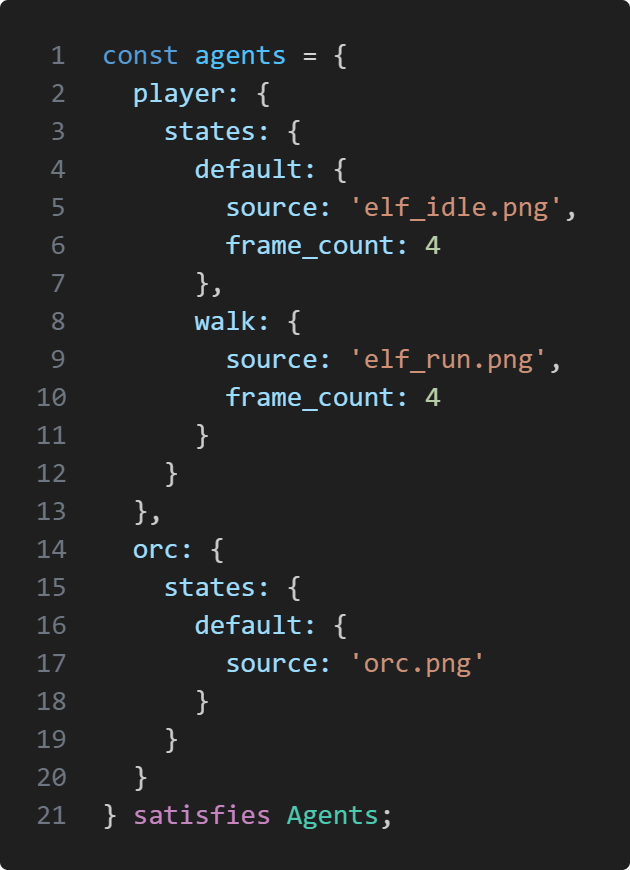
\includegraphics[width=1\textwidth]{agents.png}
        \captionof{figure}{Example Agents object}
        \label{fig:figure3}
    \end{minipage}
    
    \item \textbf{Variables:} These are custom variables that can be defined and manipulated by the developer via using Events.\\\\ \todo{refer Events}
    \begin{minipage}{\linewidth}
        \centering
        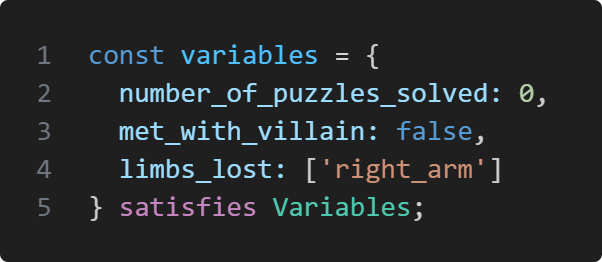
\includegraphics[width=1\textwidth]{variables.png}
        \captionof{figure}{Example Variables object}
        \label{fig:figure4}
    \end{minipage}
    
    \item \textbf{Events:} An object where keys define the name of the event, and values the sequence of actions (an array of arrays). An action is an array of keywords and primitive values such as strings, numbers or booleans. These values should be placed in a specific order, or the program will return a compiler error, pointing out the wrongly placed tokens. If placed correctly and required conditions are met during the game, the array of actions gets executed in order and synchronously, meaning the action will be fired once the previous action is completed.\\\\ 
        \begin{minipage}{\linewidth}
        \centering
        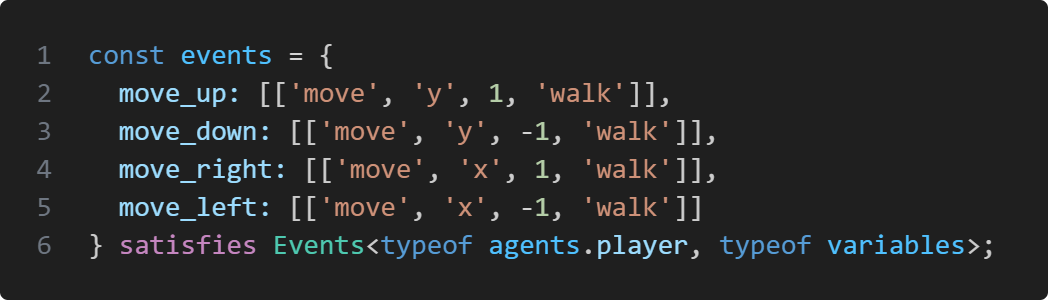
\includegraphics[width=1\textwidth]{events.png}
        \captionof{figure}{Example Events object}
        \label{fig:figure5}
    \end{minipage}
    
    \item \textbf{Key Bindings:} key bindingsss\todo{keyb} \\\\
    \begin{minipage}{\linewidth}
        \centering
        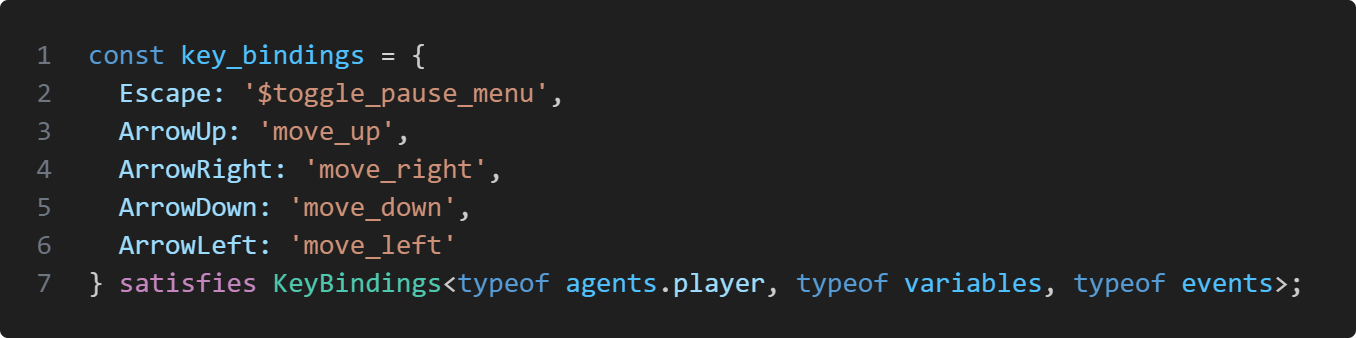
\includegraphics[width=1\textwidth]{key bindings.png}
        \captionof{figure}{Example Key Bindings object}
        \label{fig:figure6}
    \end{minipage}
    
    \item \textbf{GUI:} GUI (Graphical User Interface) \todo{gui} \\\\
    \begin{minipage}{\linewidth}
        \centering
        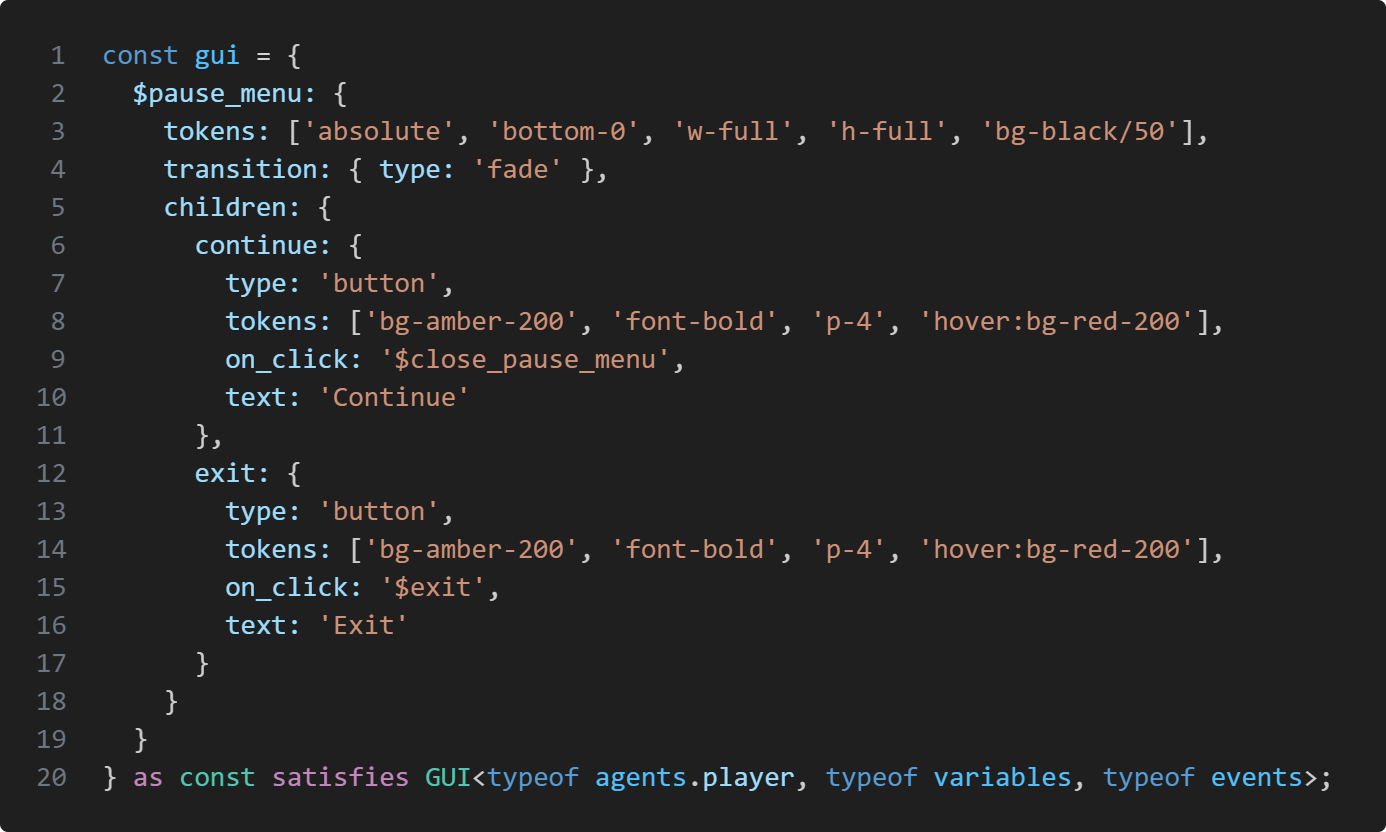
\includegraphics[width=1\textwidth]{gui.png}
        \captionof{figure}{Example GUI object}
        \label{fig:figure6}
    \end{minipage}
    
    \item \textbf{Errors}
\end{itemize}
\subsubsection{Views}
\textbf{Code Editor}
\textbf{Map Editor}
\textbf{Renderer}
\subsubsection{Exports}

\subsection{Website}
\subsubsection{Documentation}
\subsubsection{Interactive Tutorial}

\section{Conclusion}
\subsection{Future Work}
\printbibliography
\listoffigures
\end{document}
